In this section we outline the graph hamiltonicity. Recall $\F_\msf{zk}$ from Section~\ref{sec:commitment}.
$\F_\msf{zk}$ relies on some arbitrary NP relation that can be checked given an instance of a problem and a witness.  

In this section we highlight a zero knowledge protocol that can be built on top of a cryptographic commitment.
The commitment used for this example is more involved than the \Fcom presented in the main body of the paper.
The primary difference is that this \Fcom also possesses an arbitrary message-passing functionality.
It is an important feature as protocols relying on commitment often need a communication channel as well.

We modify the commitment protocol and the simulator for commitment to accomodate this additional functionality. 

\subsection{Commitment With Message Passing}
The types of the channels for this version of \Fcom are summarized before. The type and ordering for the committer and receiver are the same,
but additional labels, for each type, are added to send and receive arbitrary messages. 
\begin{tabbing}
    $\mi{type} \; \m{sender}[a]\{n\} = \ichoice{$\=$ \textcolor{red}{\paypot^2} \mb{Commit}: \m{Int} \product \m{scommitted}[a]\{n\},$ \\
    \>$\textcolor{red}{\paypot^1} \mb{Sendmsg}: \m{a} \product \m{sender}[a]\{n\}}$ \\
    $\mi{senderf2p}[a]\{n\} = \echoice{ \textcolor{red}{\getpot^1} \mb{Recvmsg}: \m{a} \arrow \m{senderf2p}}$
\end{tabbing}
The $\m{Sendmsg}$ label exist along side the other label $\mb{Open}$ as well.
Similarly, the receiver session type from the functionality is edited to add a recvmsg.
\begin{tabbing}
    $\mi{type} \; \m{receiver}[a]\{n\} = \echoice{$\=$\textcolor{red}{\getpot^0} \mb{Commit}: \m{rcommitted}[a]\{n\},$ \\
    \>$\textcolor{red}{\getpot^1} \mb{Recvmsg}: \m{a} \arrow \m{receiver}[a]\{n\}}$ \\
    $\mi{type} \; \m{receiverp2f}[a]\{n\} = \ichoice{\textcolor{red}{\paypot^1} \mb{Sendmsg}: \m{a} \product \m{receiverp2f}[a]\{n\}}$
\end{tabbing}
Finally, the adversary has a special message to get leaked messages from \Fcom:
\begin{tabbing}
    $\mi{type} \; \m{adv}[a] = \ichoice{ \mb{getLeak}: \echoice{$\=$\mb{yes}: \m{a} \arrow \m{adv}[a],$ \\
    \>$\mb{no}: \m{adv}[a]}}$
\end{tabbing}

The protocol $\pi_\msf{com}$ changes in subtle ways. Primarly, the messages they exchange over the channel functionality
is of type 
\begin{lstlisting}[basicstyle=\footnotesize\BeraMonottFamily, frame=single, mathescape]
$\Type$ commsg[a] = Commit | Open Int Int | Msg a 
\end{lstlisting}
This way there is differentiation of messages for both $\Sim_\msf{com}$ and $\pi_\msf{com}$ to know when to output received messages.
Because of this simple change, $\Sim_\msf{com}$ for the corrupt sender, from the main body of the paper, changes only slightly
to accept messages from the enviroment asking for new message leaks from the ideal functionality:
\begin{lstlisting}[basicstyle=\footnotesize\BeraMonottFamily, frame=single, mathescape]
Z2A2F,*,* =>
  $\nget$ {2} K $\$$z_to_a ;
  let m = $\nrecv$ $\$$z_to_a ;
  $\ncase$ m (
    GetLeak =>
      $\$$a_to_f.A2F ;
      $\nsend$ $\$$a_to_f GetLeak ;
      $\ncase$ $\$$a_to_f (
        yes => m = $\nrecv$ $\$$a_to_f ;
               $\$$a_to_z.F2AZ ; $\nsend$ $\$$a_to_z m ;
        no => ()
      )
      $\$$ch <- sim_com_sender[K][K1] <- (* args *) 
    $\tg{(* rest of the cases *)}$
\end{lstlisting}

\subsection{ZK Hamiltonian Cycle}
A zero-knowledge proof of the Hamiltonian Cycle relation is the canonical example of a zk-proof
that can be constructed in UC out of \Fcom~\cite{uccommitments}.

The protocol $\pi_\msf{hampath}$ and the functionality \Fzk rely on a relation checker for a graph
and a possible hamiltonian path. We give the type definition of the process that checks this relation:
\begin{lstlisting}[basicstyle=\footnotesize\BeraMonottFamily, frame=single, mathescape]
$\yo{type}$ Vertex = Int ;
$\yo{type}$ Edge = (Vertex, Vertex) ;
$\yo{type}$ Graph = (Vertex, [Edge]) ; 

$\yo{type}$ zk_relation[a][b] = &{ pair: a $\rightarrow$ b $\rightarrow$ 
  +{ yes: 1, no: 1}}

$\nproc$ ham_relation : . 
  $\vdash$ ($\$$R: zk_relation[Graph][[Edge]]) =
{
  $\ncase$ $\$$R(
    pair =>
      (* v = check the ham cycle *)
      $\nif$ v $\nthen$
        $\$$R.yes ;
      $\nelse$
        $\$$R.no ;
      $\nend$
  )
}
\end{lstlisting}

The hamiltonian path zero knowledge proof protocol uses the multisession extension of \Fcom, $!\Fcom$,
for in order to perform multiple commitments. Notice the type for a party communicating with $!\Fcom$ in 
the type definition of $\pi_\msf{hampath}$ below.
Recall that when wrapped in the multisession wrapper type, the messages from the $\pi_\msf{hampath}$ to $!\Fcom$
passes functional types without ordering even though within \Fcom the session type is being used.
The types that the typedef of $\pi_\msf{hampath}$ are the following (notice they are functional type equivalents of the session types we're seen already):
\begin{lstlisting}[basicstyle=\footnotesize\BeraMonottFamily, frame=single, mathescape]
type comp2f[a] = Commit of Bit | Open | Send of a ;
type comf2p[a] = Commit | Open of Bit | Recv of a ;
type coma2f[a] = GetLeak ;
type comf2a[a] = Yes of a | No ;
\end{lstlisting}

\begin{figure*}
\centering
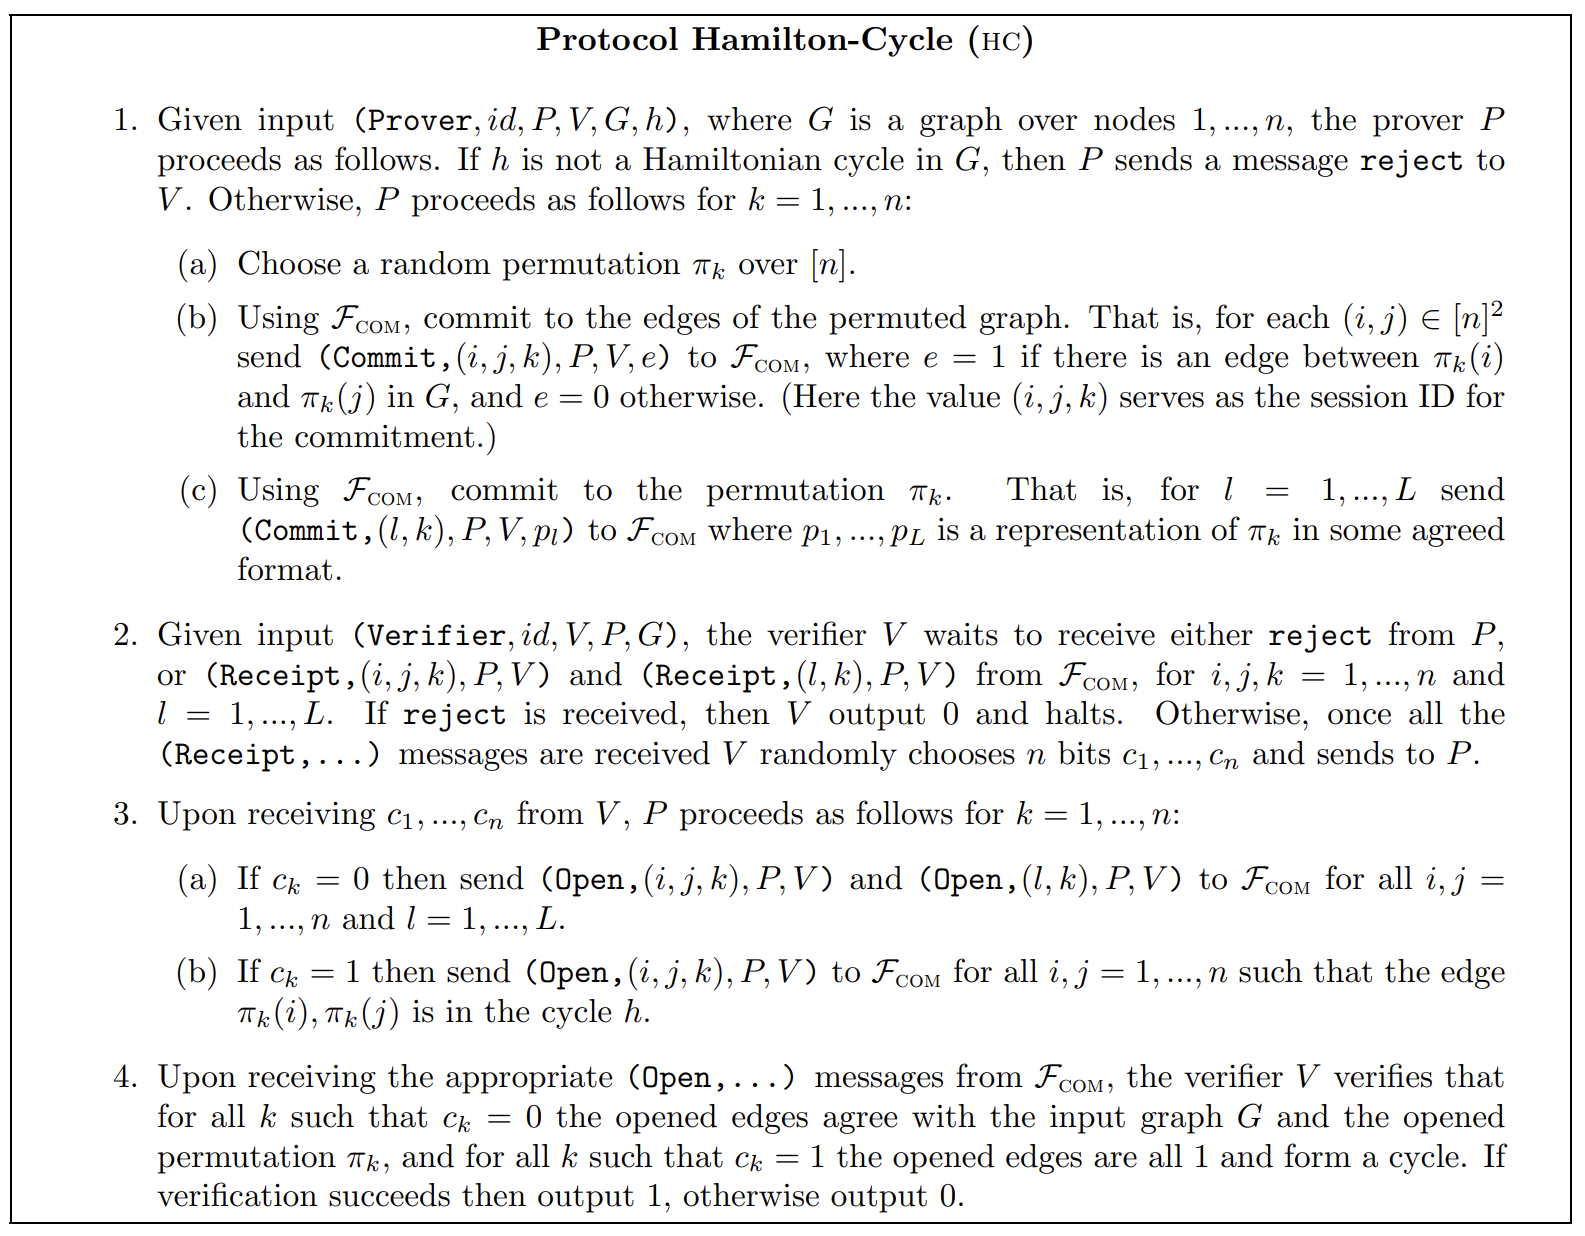
\includegraphics[scale=0.25]{figures/hampathprot.png}
\caption{The UC protocol for a zk-Hamiltonian Cycle protocol in the \Fcom-hybrid world.}
\label{fig:hampathzk}
\end{figure*}

Roughly, the protocol proceeds as follows, and is detailed in Figure~\ref{fig:hampathzk}.
If the hamiltonian cycle given by \Z to the prover passes \inline{ham_relation} it create $k \in \{1..n\}$ different
permutation $\pi_k$ of the nodes and for each one, it creates a commitment for every pair of nodes $i,j$ and creates $n^3$ commitments
where the \m{ssid} is $(i,j,k)$ as detailed by $\inline{ham_sid}$ below. The bit being committed to
is the whether $\pi_k(i)$ and $\pi_k(j)$ have an edge in the original graph. 
Finally the prover commits to each of the $k$ permutations of the graph.  
The verifier selects a series of the $n$ bits which determines, out of the $k$ permutations whether
the open the commitment to the the whole permutation or or open the commitment to the edges that form a cycle
in the permutation. 
The verifier performs the checks described in Figure~\ref{fig:hampathzk}


We detail how the prover code. First we highlight the type for the prover and the verifier.
\begin{tabbing}
    $\mi{type} \; \m{prover}[a]\{n\} = \ichoice{$\=$ \textcolor{red}{\paypot^n} \mb{Commitment}: a \product$ \\ 
    \>$\echoice{ \mb{Yes}: 1, \mb{No}: 1 }}$ \\
    $\mi{type} \; \m{verifier}[a,b]\{n\} = \ichoice{ \textcolor{red}{\paypot^n} \mb{witness}: a \product b \product \m{activate}[a,b]\{n\}}$ \\
    $\mi{type} \; \m{activate}\{n\} = \ichoice{ \textcolor{red}{\paypot^n} \mb{domore}: \m{activate}\{n\}}$
\end{tabbing}

The pro
The prover code for hamiltonian path that sends commitments to $!\Fcom$:
\begin{lstlisting}[basicstyle=\footnotesize\BeraMonottFamily, frame=single, mathescape]
type ham_sid = (Int, Int, Int)

$\nproc$ prot_ham_prover :
  (k: Int), (rng: [Bit]), (sid: session[1]),
  ($\$$z2p: prover[Graph][[Edge]]), ($\$$p2z: 1), 
  ($\$$p2f: p2ms[ham_sid][comp2f]{2}), ($\$$f2p: p2ms[ham_sid][comf2p]{0}) |- ($\$$ch: 1) =
{
  $\ncase$ $\$$z2p (
    witness =>
      $\nget$ \{3\} K $\$$z2p ;
      graph = $\nrecv$ $\$$z2p ; hpath = $\nrecv$ $\$$z2p ;
      $\$$R <- ham_relation <- ;
      $\$$R.pair ; $\nsend$ $\$$R (graph, hpath) ;
      $\ncase$ $\$$R (
        yes => 
          let n = size graph ;
          $\nfor$ k in [1..n] $\nthen$
            $\$$p <- graph_permute ;
            $\$$p.permute ; $\nsend$ $\$$p graph ;
            $\ncase$ $\$$p ( permutation =>
              let newnodes = recv $\$$p ;
              $\nfor$ i in [1..n] $\nthen$
                $\nfor$ j in [1..n] $\nthen$
                  let ssid = (i, j, k)
                  let pi = geti newnodes i
                  let pj = geti newnodes j
                  let e = isedge graph pi pj 
                  $\$$p2ms.p2bf ; $\npay$ \{2\} ;
                  $\nsend$ $\$$p2ms ssid ;
                  $\nsend$ $\$$p2ms (Commit e) ;
                  $\nif$ (j<n) $\nthen$
                    $\ncase$ $\$$z2p ( domore => 
                      $\nget$ {3} K $\$$z2p; )
                  $\nelse$ ()
                $\nend$
                $\nif$ (i<n) $\nthen$
                  $\ncase$ $\$$z2p ( domore => 
                    $\nget$ {3} K $\$$z2p; )
                $\nelse$ ()
              $\nend$
            )
          $\nif$ (k<n) $\nthen$
            $\ncase$ $\$$z2p ( domore => $\nget$ {3} K $\$$z2p; )
          $\nelse$ ()
        no => 
          $\tg{* reject input *)}$
      )
  )
}
\end{lstlisting}

The type of the simulator is straightforward and makes sense given the type of the protocol above. It
relies on some generic template types we haven't seen yet:

\begin{lstlisting}[basicstyle=\footnotesize\BeraMonottFamily, frame=single, mathescape]
$\nproc$ sim_ham_prover[K][K1] :
  (k: Int), (rng: [Bit]), (sid: session[1]),
  ($\$$z_to_a: z2a[K][p2ms[comp2f]][a2ms[coma2f]]{3}), 
  ($\$$a_to_z: a2z[K][ms2p[comf2p]][ms2a[coma2f]]{0}),
  ($\$$p_to_a: p2a[K][zkp2f]{3}), ($\$$a_to_p: a2p[K][zkp2f]{3}), 
  ($\$$a_to_f: zka2f{1}), ($\$$f_to_a: zkf2a{0}),
  ($\$commitment: [Edge]) |- ($\$$c: 1)
\end{lstlisting}

The type of this simulator indicates that it accepts messages from \Z for corrupt protocol parties
according to the real world ideal functionality $!\Fcom$. Therefore, messages are wrapped in the 
\inline{p2ms} type mentioned. 

When composing two protocols, we are already guarantees that the types of protocol being swapped in for the functionality is identical. 
This include the import exchanged as well. 
Recall that composition operator in Section~\ref{sec:execuc}. Applying the operator to the protocol above with $\pi_\msf{com}$ is quite straightforward as the tokens exchanged are the same.
Similarly, composing simulators is trivial as we simply take output for the protocol parties and $\Fcom$ from $\Sim_\msf{com}$ and casts it as \inline{z2p} input for $\Sim_\msf{hampath}$ using an operator as generic as the composition operator itself.
